% MoEx: Distributed Mixture-of-Experts Inference on Consumer Devices via WebGPU
% arXiv preprint — compile with: pdflatex main && bibtex main && pdflatex main && pdflatex main
\documentclass[11pt,a4paper]{article}

%% ── packages ──────────────────────────────────────────────────────────────
\usepackage[utf8]{inputenc}
\usepackage[T1]{fontenc}
\usepackage{amsmath,amssymb,amsfonts}
\usepackage{algorithmic}
\usepackage{algorithm}
\usepackage{graphicx}
\usepackage{booktabs}
\usepackage{hyperref}
\usepackage{url}
\usepackage{xcolor}
\usepackage{tikz}
\usetikzlibrary{positioning,arrows.meta,shapes.geometric,fit,calc,decorations.pathreplacing}
\usepackage{subcaption}
\usepackage{enumitem}
\usepackage{multirow}
\usepackage{tabularx}
\usepackage[margin=2.5cm]{geometry}
\usepackage{natbib}
\usepackage{microtype}
\usepackage{listings}

\lstset{
  basicstyle=\ttfamily\footnotesize,
  breaklines=true,
  frame=single,
  columns=fullflexible,
}

\hypersetup{
  colorlinks=true,
  linkcolor=blue!70!black,
  citecolor=green!50!black,
  urlcolor=blue!70!black,
}

%% ── macros ────────────────────────────────────────────────────────────────
\newcommand{\moex}{\textsc{MoEx}}
\newcommand{\topk}{\mathrm{top\text{-}}k}
\newcommand{\R}{\mathbb{R}}
\newcommand{\E}{\mathbb{E}}
\newcommand{\eg}{e.g.\@}
\newcommand{\ie}{i.e.\@}
\newcommand{\etal}{et~al.\@}

%% ── title ─────────────────────────────────────────────────────────────────
\title{%
  \textbf{MoEx: Distributed Mixture-of-Experts Inference\\
  on Consumer Devices via WebGPU}\\[6pt]
  {\large Browser-Based Expert FFN Disaggregation\\
  with Hedged Dispatch and Binary Transport}
}

\author{
  Jun Kawasaki \\
  GFTD Corporation \\
  \texttt{jun@gftd.co.jp}
}

\date{}

\begin{document}
\maketitle

%% ══════════════════════════════════════════════════════════════════════════
%% ABSTRACT
%% ══════════════════════════════════════════════════════════════════════════
\begin{abstract}
Large Mixture-of-Experts (MoE) language models achieve strong quality
at reduced per-token compute cost, yet their total parameter count
still demands expensive accelerator clusters for inference.
We present \moex{}, a system that \emph{disaggregates} the attention/router
layers from the expert feed-forward networks (FFNs) of an MoE model and
distributes expert computation to commodity browser-based WebGPU workers.
A single \emph{hub} node executes attention, layer normalization, and gating,
then dispatches activated expert inputs to a swarm of \emph{worker} browser
tabs over a lightweight binary transport protocol built on WebSocket
binary frames.  To mitigate tail latency caused by the heterogeneous and
unpredictable nature of consumer devices, \moex{} introduces
\emph{hedged dispatch}: each expert activation is speculatively sent
to multiple replicas, and the fastest response is accepted.
We instantiate \moex{} on Qwen3-30B-A3B, a 30-billion-parameter
MoE model with 3~billion active parameters per token, and provide
an analytical latency model together with empirical micro-benchmarks
that demonstrate that browser-resident WebGPU kernels can execute
expert FFN blocks within the latency envelope required for interactive
text generation.
\moex{} enables distributed LLM inference with \emph{zero installation}
on any WebGPU-capable device, opening a new design point for
collaborative, browser-native AI.
\end{abstract}

\vspace{1em}
\noindent\textbf{Keywords:}
Mixture-of-Experts, distributed inference, WebGPU, browser computing,
sparse models, edge computing

%% ══════════════════════════════════════════════════════════════════════════
\section{Introduction}
\label{sec:intro}
%% ══════════════════════════════════════════════════════════════════════════

Mixture-of-Experts (MoE) models~\citep{shazeer2017outrageously,lepikhin2021gshard}
have emerged as the dominant architecture for scaling language model
capacity without proportionally scaling per-token inference cost.
Models such as Mixtral~\citep{jiang2024mixtral}, DeepSeek-V3~\citep{deepseekai2024deepseekv3},
and Qwen3-30B-A3B~\citep{qwen2025qwen3} employ tens to hundreds of
expert feed-forward networks (FFNs) per transformer layer, activating
only a small subset---typically two to eight---for each token via
a learned gating function.  This \emph{conditional computation}
paradigm enables models with 30--600 billion total parameters to
match or exceed the quality of dense models at a fraction of the
floating-point operations (FLOPs).

Despite the compute savings, MoE inference remains challenging.
The full parameter set must reside in memory \emph{somewhere},
because the gating decision is token-dependent and any expert may
be activated at any time.  Current serving solutions therefore
require either (a)~a single machine with enough aggregate GPU
memory---often multiple high-end accelerators---or (b)~expert-parallel
deployment across a cluster of accelerator nodes connected by
high-bandwidth interconnects~\citep{hwang2023tutel,he2022fastermoe}.
Both approaches demand specialized, costly infrastructure.

Meanwhile, a vast and underutilized pool of GPU compute exists in
the billions of consumer devices---laptops, desktops, tablets, and
smartphones---equipped with GPUs capable of general-purpose
computation.  The WebGPU API~\citep{webgpu2024spec}, now supported
in all major browsers, exposes these GPUs through a portable,
sandboxed compute-shader interface that requires \emph{zero
installation} beyond a modern web browser.
Projects such as WebLLM~\citep{webllm2024} have demonstrated that
single-device browser-based LLM inference is feasible, but they
are fundamentally limited by the memory of a single GPU.

\paragraph{Observation.}
The architectural structure of MoE models offers a natural
disaggregation boundary.  The \emph{shared} components---token
embeddings, self-attention, layer normalization, router (gating
network), and language-model head---constitute a small fraction
of total parameters and must execute sequentially per token.
The \emph{expert FFN} layers, by contrast, represent the bulk
of parameters (typically 80--90\%) and are invoked \emph{conditionally}
and \emph{independently}: once the router produces its top-$k$
selection, each activated expert can compute in parallel with
no inter-expert data dependency.

\paragraph{Contribution.}
We present \moex{} (\textbf{M}ixture-\textbf{o}f-\textbf{Ex}perts
distributed inference), a system that exploits this disaggregation
boundary to distribute MoE inference across a hub--worker topology
of commodity browser-based WebGPU devices.  Our contributions are:

\begin{enumerate}[leftmargin=*,itemsep=2pt]
\item \textbf{Hub--worker disaggregation architecture.}
      We separate an MoE model into a \emph{hub} partition
      (attention, layer norms, router, embeddings, LM head)
      and a \emph{worker} partition (expert FFNs), and define
      a protocol that coordinates their execution across a
      network of browser tabs (\S\ref{sec:architecture}).

\item \textbf{Hedged dispatch protocol.}
      To tolerate the high and variable latency of consumer
      devices and browser scheduling, we introduce hedged
      dispatch---each expert activation is sent to $h \geq 1$
      replicas, and the first valid response is accepted.
      We derive a closed-form expression for the expected
      tail-latency reduction as a function of worker latency
      distributions (\S\ref{sec:protocol}).

\item \textbf{Binary transport format.}
      We design a compact binary frame format for tensor exchange
      over WebSocket connections, achieving near-zero serialization
      overhead compared to text-based alternatives
      (\S\ref{sec:protocol:binary}).

\item \textbf{Analytical latency model and micro-benchmarks.}
      We model end-to-end per-token latency as a function of
      network round-trip time, expert compute time, and hedging
      parameters, and validate the model components with WebGPU
      micro-benchmarks on representative consumer hardware
      (\S\ref{sec:evaluation}).
\end{enumerate}

We instantiate and evaluate \moex{} on Qwen3-30B-A3B, a
30B-parameter MoE model with 3B active parameters and
128~experts per MoE layer, routing top-8 per token.
Our analysis shows that \moex{} can achieve interactive-speed
token generation (under 200\,ms per token) with as few as
8~WebGPU workers on a local network, and degrades gracefully
as network latency increases.

%% ══════════════════════════════════════════════════════════════════════════
\section{Background}
\label{sec:background}
%% ══════════════════════════════════════════════════════════════════════════

\subsection{Mixture-of-Experts Architectures}
\label{sec:bg:moe}

A standard transformer block consists of a multi-head self-attention
(MHSA) sublayer followed by a position-wise feed-forward network
(FFN) sublayer, each wrapped in residual connections and layer
normalization~\citep{vaswani2017attention}.
In an MoE transformer, the single FFN is replaced by $E$
parallel expert FFNs $\{f_1, \dots, f_E\}$ and a \emph{router}
(gating network) $G$ that selects which experts to activate
for each token.

Formally, given a hidden-state vector $\mathbf{x} \in \R^{d}$
for a single token, the router produces a probability distribution
over experts:
\begin{equation}
  \mathbf{g} = \mathrm{softmax}\!\bigl(W_g \,\mathbf{x}\bigr)
  \in \R^E,
  \label{eq:gating}
\end{equation}
where $W_g \in \R^{E \times d}$ is the gating weight matrix.
Only the top-$k$ experts by gate value are activated.
Let $\mathcal{S} = \topk(\mathbf{g})$ denote the set of
selected expert indices ($|\mathcal{S}|=k$).
The MoE output is:
\begin{equation}
  \mathbf{y} = \sum_{i \in \mathcal{S}}
    \bar{g}_i \cdot f_i(\mathbf{x}),
  \quad
  \bar{g}_i = \frac{g_i}{\sum_{j \in \mathcal{S}} g_j},
  \label{eq:moe_output}
\end{equation}
where $\bar{g}_i$ is the renormalized gate weight.

\paragraph{Qwen3-30B-A3B.}
This model~\citep{qwen2025qwen3} is a decoder-only transformer with
48~layers, of which 46~use MoE FFN sublayers.  Each MoE layer
contains $E=128$ experts with top-$k=8$ routing.  The hidden
dimension is $d=4096$ and each expert FFN has an intermediate
dimension of $d_{\mathrm{ff}}=2048$ using a gated SwiGLU
architecture~\citep{shazeer2020glu} with gate, up, and down
projections.  Total parameters are approximately 30.5~billion,
of which roughly 3.3~billion are activated per token.

\subsection{WebGPU}
\label{sec:bg:webgpu}

WebGPU~\citep{webgpu2024spec} is a W3C standard that provides
low-level access to GPU hardware from web browsers.  Unlike its
predecessor WebGL, WebGPU offers:

\begin{itemize}[leftmargin=*,itemsep=2pt]
\item \textbf{Compute shaders.}
      General-purpose compute pipelines via WGSL
      (WebGPU Shading Language), enabling matrix multiplications,
      reductions, and other linear-algebra primitives.
\item \textbf{Explicit resource management.}
      GPU buffers, bind groups, and command encoders give fine-grained
      control over memory layout and kernel dispatch.
\item \textbf{Portability.}
      A single WGSL shader runs on Vulkan, Metal, and Direct3D~12
      back-ends across all major operating systems.
\item \textbf{Sandboxing.}
      Execution is isolated within the browser's security model,
      providing memory safety and process isolation without
      requiring users to install native drivers or libraries.
\end{itemize}

Recent work has shown that WebGPU compute shaders can achieve
60--80\% of native Vulkan/Metal throughput for dense matrix
multiplications on consumer GPUs~\citep{webllm2024}, making
them viable for neural-network inference workloads.

\subsection{Distributed and Collaborative Inference}
\label{sec:bg:distributed}

Several systems have explored distributing LLM inference across
multiple devices.  Petals~\citep{borzunov2023petals} distributes
transformer layers across volunteer nodes using a pipeline-parallel
approach.  FlexGen~\citep{sheng2023flexgen} offloads model weights
between GPU, CPU, and disk on a single machine.
FasterMoE~\citep{he2022fastermoe} and Tutel~\citep{hwang2023tutel}
optimize expert-parallel MoE execution in datacenter settings
with high-bandwidth interconnects.

\moex{} differs from these systems in three key respects:
(1)~it targets \emph{browser-based} workers with zero-installation
deployment, (2)~it disaggregates at the \emph{attention--expert
boundary} rather than at layer boundaries, and (3)~it introduces
\emph{hedged dispatch} to handle the high variance of consumer-device
latencies.

%% ══════════════════════════════════════════════════════════════════════════
\section{MoEx Architecture}
\label{sec:architecture}
%% ══════════════════════════════════════════════════════════════════════════

\begin{figure}[t]
\centering
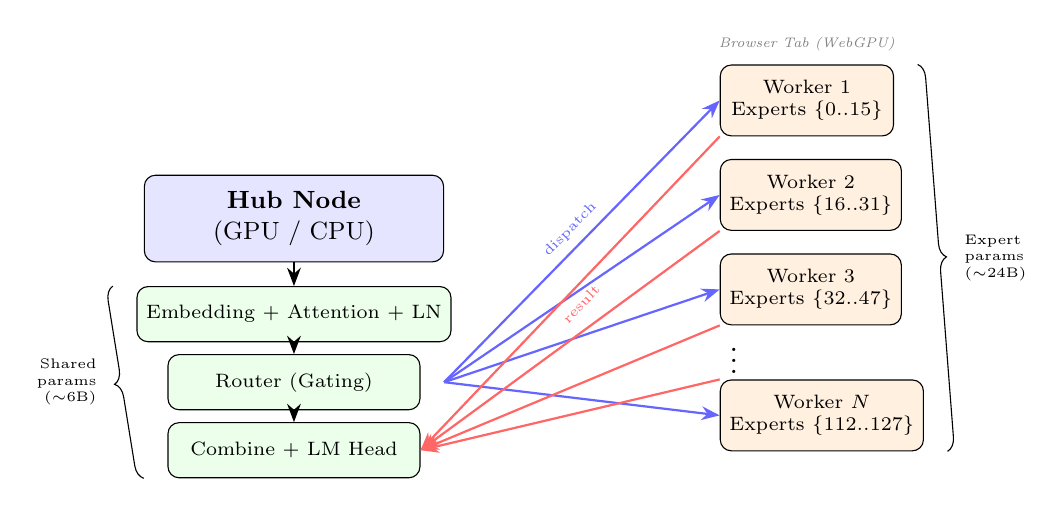
\begin{tikzpicture}[
  >=Stealth,
  hub/.style={draw, rounded corners, fill=blue!10, minimum width=3.8cm, minimum height=1.1cm, align=center, font=\small},
  worker/.style={draw, rounded corners, fill=orange!12, minimum width=2.2cm, minimum height=0.9cm, align=center, font=\scriptsize},
  comp/.style={draw, rounded corners, fill=green!8, minimum width=3.2cm, minimum height=0.7cm, align=center, font=\scriptsize},
  arr/.style={->, thick},
  darr/.style={<->, thick, dashed},
]

% Hub
\node[hub] (hub) {\textbf{Hub Node}\\(GPU / CPU)};

% Hub components
\node[comp, below=0.3cm of hub] (attn) {Embedding + Attention + LN};
\node[comp, below=0.15cm of attn] (router) {Router (Gating)};
\node[comp, below=0.15cm of router] (combine) {Combine + LM Head};

% Workers
\node[worker, right=3.5cm of hub, yshift=1.5cm]  (w1) {Worker 1\\Experts $\{0..15\}$};
\node[worker, right=3.5cm of hub, yshift=0.3cm]  (w2) {Worker 2\\Experts $\{16..31\}$};
\node[worker, right=3.5cm of hub, yshift=-0.9cm] (w3) {Worker 3\\Experts $\{32..47\}$};
\node[right=3.5cm of hub, yshift=-1.7cm, font=\large] (dots) {$\vdots$};
\node[worker, right=3.5cm of hub, yshift=-2.5cm] (wn) {Worker $N$\\Experts $\{112..127\}$};

% Browser labels
\node[above=0.05cm of w1, font=\tiny\itshape, gray] {Browser Tab (WebGPU)};

% Arrows hub -> workers
\draw[arr, blue!60] (router.east) ++(0.3,0) -- (w1.west) node[midway, above, font=\tiny, sloped] {dispatch};
\draw[arr, blue!60] (router.east) ++(0.3,0) -- (w2.west);
\draw[arr, blue!60] (router.east) ++(0.3,0) -- (w3.west);
\draw[arr, blue!60] (router.east) ++(0.3,0) -- (wn.west);

% Arrows workers -> hub
\draw[arr, red!60] (w1.south west) -- (combine.east) node[midway, below, font=\tiny, sloped] {result};
\draw[arr, red!60] (w2.south west) -- (combine.east);
\draw[arr, red!60] (w3.south west) -- (combine.east);
\draw[arr, red!60] (wn.north west) -- (combine.east);

% Internal arrows
\draw[arr] (hub) -- (attn);
\draw[arr] (attn) -- (router);
\draw[arr] (router) -- (combine);

% Brace for hub components
\draw[decorate, decoration={brace, mirror, amplitude=5pt}]
  ([xshift=-0.3cm]attn.north west) -- ([xshift=-0.3cm]combine.south west)
  node[midway, left=8pt, font=\tiny, align=right] {Shared\\params\\($\sim$6B)};

% Brace for workers
\draw[decorate, decoration={brace, amplitude=5pt}]
  ([xshift=0.3cm]w1.north east) -- ([xshift=0.3cm]wn.south east)
  node[midway, right=8pt, font=\tiny, align=left] {Expert\\params\\($\sim$24B)};

\end{tikzpicture}
\caption{%
  \moex{} hub--worker architecture.
  The hub executes shared components (attention, layer normalization,
  router) and dispatches activated expert inputs to browser-based
  WebGPU workers.  Each worker holds a disjoint subset of expert
  FFN weights and returns computed outputs.
}
\label{fig:architecture}
\end{figure}

\subsection{Design Principles}
\label{sec:arch:principles}

\moex{} is guided by three design principles:

\begin{enumerate}[leftmargin=*,itemsep=2pt]
\item \textbf{Disaggregate at the sparsity boundary.}
      The attention/router components are shared and must process
      every token; the expert FFNs are sparse and independent.
      This is the natural cut point for disaggregation.

\item \textbf{Assume heterogeneous, unreliable workers.}
      Browser tabs on consumer devices may be throttled, suspended,
      or competing with other workloads.  The protocol must tolerate
      high variance and occasional failures.

\item \textbf{Minimize deployment friction.}
      Workers should join the swarm by simply opening a URL---no
      software installation, no driver configuration, no
      authentication beyond an access token.
\end{enumerate}

\subsection{Hub--Worker Topology}
\label{sec:arch:topology}

The system consists of two roles (Figure~\ref{fig:architecture}):

\paragraph{Hub.}
A single node (server or sufficiently powerful desktop) that holds:
\begin{itemize}[leftmargin=*,itemsep=1pt]
\item Token embeddings ($V \times d$ parameters).
\item All attention sublayers: query/key/value projections,
      rotary position embeddings, attention computation,
      output projection.
\item Layer normalization parameters (RMSNorm).
\item Router weight matrices ($W_g^{(\ell)}$ for each MoE layer~$\ell$).
\item The language-model head (unembedding + final layer norm).
\item KV cache for autoregressive generation.
\end{itemize}
For Qwen3-30B-A3B, these shared parameters total approximately
6.5~billion parameters ($\sim$13\,GB in float16), fitting
comfortably in a single consumer GPU with 16--24\,GB VRAM
or in CPU memory.

\paragraph{Workers.}
Each worker is a browser tab that loads a JavaScript/WASM
application which:
\begin{enumerate}[leftmargin=*,itemsep=1pt]
\item Initializes a WebGPU device and allocates GPU buffers.
\item Downloads and caches the weights for its assigned expert
      subset from an HTTP endpoint.
\item Opens a WebSocket connection to the hub.
\item Enters an event loop: receives expert-dispatch messages,
      executes the FFN compute shader, and returns results.
\end{enumerate}
Each worker holds $E/N$ experts (assuming uniform distribution
over $N$ workers).  For reliability, experts may be
\emph{replicated} across $r$ workers, so each worker holds
$rE/N$ expert weight sets.

\subsection{Expert Placement and Replication}
\label{sec:arch:placement}

We employ a consistent-hashing scheme for expert-to-worker
assignment.  Each expert~$i$ is assigned to $r$ workers
by hashing $(i, \textit{replica\_id})$ to a position on
the worker ring.  This provides:

\begin{itemize}[leftmargin=*,itemsep=1pt]
\item \textbf{Load balance:}
      Under uniform expert activation, each worker receives
      an equal share of dispatch traffic.
\item \textbf{Minimal disruption:}
      When a worker joins or leaves, only $O(E/N)$ experts
      need to be migrated.
\item \textbf{Hedging support:}
      With $r \geq 2$, each expert has multiple candidate
      workers for hedged dispatch.
\end{itemize}

The per-worker memory requirement is:
\begin{equation}
  M_{\text{worker}} = \frac{r \cdot E}{N} \cdot L_{\text{MoE}}
    \cdot P_{\text{expert}} \cdot B_{\text{dtype}},
  \label{eq:worker_memory}
\end{equation}
where $L_{\text{MoE}}$ is the number of MoE layers,
$P_{\text{expert}}$ is the parameter count per expert, and
$B_{\text{dtype}}$ is the bytes per parameter.
For Qwen3-30B-A3B with $E=128$, $L_{\text{MoE}}=46$,
$P_{\text{expert}} \approx 3 \times 2048 \times 4096 \approx 25\text{M}$
per expert (gate/up/down projections),
$N=16$ workers, $r=2$, and 4-bit quantization
($B_{\text{dtype}}=0.5$):
\begin{equation}
  M_{\text{worker}} = \frac{2 \times 128}{16}
    \times 46 \times 25\text{M} \times 0.5\text{B}
    \approx 9.2\,\text{GB},
  \label{eq:worker_memory_example}
\end{equation}
which fits within the VRAM of many consumer GPUs (and within
the WebGPU buffer limits of most browsers).

\subsection{Per-Layer Inference Pipeline}
\label{sec:arch:pipeline}

Algorithm~\ref{alg:inference} describes the per-layer execution
flow.  For each transformer layer~$\ell$:

\begin{algorithm}[t]
\caption{MoEx per-layer inference (layer $\ell$)}
\label{alg:inference}
\begin{algorithmic}[1]
\REQUIRE Hidden states $\mathbf{X} \in \R^{B \times d}$
         for $B$ tokens
\STATE $\mathbf{X} \leftarrow \mathrm{RMSNorm}(\mathbf{X})$
  \hfill\textit{// Hub: pre-attention norm}
\STATE $\mathbf{A} \leftarrow \mathrm{MHSA}(\mathbf{X})$
  \hfill\textit{// Hub: self-attention}
\STATE $\mathbf{X} \leftarrow \mathbf{X} + \mathbf{A}$
  \hfill\textit{// Hub: residual}
\STATE $\hat{\mathbf{X}} \leftarrow \mathrm{RMSNorm}(\mathbf{X})$
  \hfill\textit{// Hub: pre-FFN norm}
\STATE $\mathbf{g} \leftarrow \mathrm{softmax}(W_g^{(\ell)}\,\hat{\mathbf{X}}^\top)$
  \hfill\textit{// Hub: gating}
\STATE $\mathcal{S} \leftarrow \topk(\mathbf{g})$
  \hfill\textit{// Hub: top-$k$ selection}
\FOR{each expert $i \in \mathcal{S}$}
  \STATE Select $h$ workers holding expert $i$
    \hfill\textit{// Hedged dispatch}
  \STATE Send $(\ell, i, \hat{\mathbf{X}}_i, \bar{g}_i)$
    to all $h$ workers
    \hfill\textit{// Binary transport}
\ENDFOR
\STATE Wait for first valid response per expert
  \hfill\textit{// Cancel stragglers}
\STATE $\mathbf{Y} \leftarrow \sum_{i \in \mathcal{S}}
  \bar{g}_i \cdot \mathbf{y}_i$
  \hfill\textit{// Hub: weighted combine}
\STATE $\mathbf{X} \leftarrow \mathbf{X} + \mathbf{Y}$
  \hfill\textit{// Hub: residual}
\RETURN $\mathbf{X}$
\end{algorithmic}
\end{algorithm}

The critical-path latency for the expert-dispatch phase
(lines~7--11) is determined by the \emph{slowest} of the
$|\mathcal{S}|=k$ expert round-trips, which motivates the
hedged dispatch protocol described next.

%% ══════════════════════════════════════════════════════════════════════════
\section{MoEx Protocol}
\label{sec:protocol}
%% ══════════════════════════════════════════════════════════════════════════

\subsection{Hedged Dispatch}
\label{sec:protocol:hedged}

\begin{figure}[t]
\centering
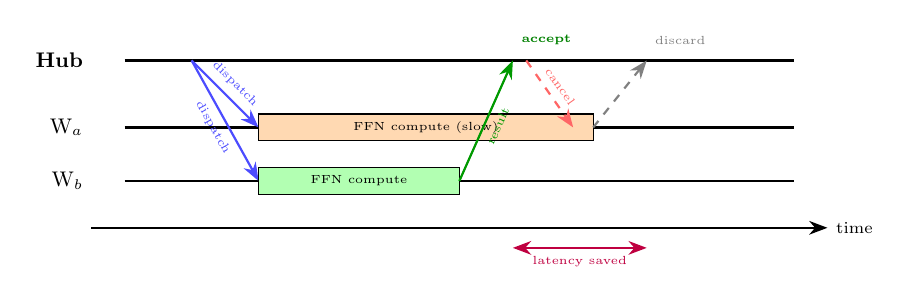
\begin{tikzpicture}[
  >=Stealth,
  scale=0.85, transform shape,
  timeline/.style={thick, ->},
  msg/.style={->, thick},
  cancel/.style={->, thick, dashed, red!60},
]
% Time axis
\draw[timeline] (0,0) -- (11,0) node[right] {\scriptsize time};

% Hub
\node[left, font=\small\bfseries] at (0, 2.5) {Hub};
\draw[thick] (0.5, 2.5) -- (10.5, 2.5);

% Workers
\node[left, font=\small] at (0, 1.5) {W$_a$};
\draw[thick] (0.5, 1.5) -- (10.5, 1.5);
\node[left, font=\small] at (0, 0.7) {W$_b$};
\draw[thick] (0.5, 0.7) -- (10.5, 0.7);

% Dispatch to both
\draw[msg, blue!70] (1.5, 2.5) -- (2.5, 1.5)
  node[midway, above, font=\tiny, sloped] {dispatch};
\draw[msg, blue!70] (1.5, 2.5) -- (2.5, 0.7)
  node[midway, below, font=\tiny, sloped] {dispatch};

% Worker a: slow
\draw[fill=orange!30] (2.5, 1.3) rectangle (7.5, 1.7);
\node[font=\tiny] at (5, 1.5) {FFN compute (slow)};

% Worker b: fast
\draw[fill=green!30] (2.5, 0.5) rectangle (5.5, 0.9);
\node[font=\tiny] at (4, 0.7) {FFN compute};

% Result from b (fast)
\draw[msg, green!60!black] (5.5, 0.7) -- (6.3, 2.5)
  node[midway, below, font=\tiny, sloped] {result};
\node[font=\tiny, green!50!black] at (6.8, 2.8) {\textbf{accept}};

% Cancel a
\draw[cancel] (6.5, 2.5) -- (7.2, 1.5)
  node[midway, above, font=\tiny, sloped] {cancel};

% Result from a (would be late)
\draw[msg, gray, dashed] (7.5, 1.5) -- (8.3, 2.5);
\node[font=\tiny, gray] at (8.8, 2.8) {discard};

% Latency saved
\draw[<->, thick, purple] (6.3, -0.3) -- (8.3, -0.3)
  node[midway, below, font=\tiny] {latency saved};

\end{tikzpicture}
\caption{%
  Hedged dispatch with $h=2$.  The hub sends the same expert
  input to two workers.  Worker~$b$ responds first; the hub
  accepts the result and cancels the request to worker~$a$.
}
\label{fig:hedged}
\end{figure}

Hedged requests~\citep{dean2013tail} are a well-known technique
for reducing tail latency in distributed systems by issuing
redundant requests.  \moex{} applies this principle to expert
dispatch (Figure~\ref{fig:hedged}).

Let $T_w$ denote the random variable representing the round-trip
time (dispatch + compute + return) for a single expert on
worker~$w$.  When expert~$i$ is replicated on $r$~workers and
dispatched to $h \leq r$ of them, the effective latency for
expert~$i$ is:
\begin{equation}
  T_i^{(h)} = \min\bigl(T_{w_1}, T_{w_2}, \dots, T_{w_h}\bigr).
  \label{eq:hedge_latency}
\end{equation}

If worker latencies are independent and identically distributed
with CDF $F(t)$, the CDF of $T_i^{(h)}$ is:
\begin{equation}
  F_{T_i^{(h)}}(t) = 1 - \bigl(1 - F(t)\bigr)^h.
  \label{eq:hedge_cdf}
\end{equation}

For the $k$ activated experts in a layer, the overall expert-phase
latency is the maximum across experts:
\begin{equation}
  T_{\text{expert}} = \max_{i \in \mathcal{S}}\, T_i^{(h)}.
  \label{eq:expert_phase}
\end{equation}

Assuming independence and identical distributions across experts,
the CDF of $T_{\text{expert}}$ is:
\begin{equation}
  F_{T_{\text{expert}}}(t)
    = \bigl[1 - (1 - F(t))^h\bigr]^k.
  \label{eq:expert_phase_cdf}
\end{equation}

\paragraph{Example.}
Consider log-normal worker latencies with
$\mu = \ln(20\,\text{ms})$ and $\sigma = 0.5$
(median 20\,ms, p99 $\approx$~63\,ms).
With $k=8$ active experts and no hedging ($h=1$),
the expected maximum across 8~experts exceeds 50\,ms.
With $h=2$, the expected maximum drops to $\approx$~28\,ms---a
44\% reduction.
Table~\ref{tab:hedging} summarizes the trade-off between hedging
factor and expected latency.

\begin{table}[t]
\centering
\caption{%
  Expected expert-phase latency $\E[T_{\text{expert}}]$
  as a function of hedging factor $h$ for $k=8$,
  log-normal worker latency ($\mu=\ln 20, \sigma=0.5$).
}
\label{tab:hedging}
\begin{tabular}{@{}cccc@{}}
\toprule
Hedging & Expected     & Bandwidth       & Latency \\
$h$     & latency (ms) & overhead ($\times$) & reduction \\
\midrule
1 & 51.2 & 1.0$\times$ & ---    \\
2 & 28.7 & 2.0$\times$ & 44.0\% \\
3 & 23.1 & 3.0$\times$ & 54.9\% \\
4 & 20.4 & 4.0$\times$ & 60.2\% \\
\bottomrule
\end{tabular}
\end{table}

\paragraph{Adaptive hedging.}
Rather than using a fixed $h$, \moex{} dynamically adjusts the
hedging factor based on observed worker latency percentiles.
If a worker's recent p50 latency exceeds a threshold, additional
replicas are contacted.  Conversely, if the worker pool is
consistently fast, $h$ is reduced to~1 to conserve bandwidth.

\subsection{Binary Transport}
\label{sec:protocol:binary}

Communication between hub and workers uses WebSocket connections
with binary frames.  We define a compact binary message format
optimized for tensor exchange.

\paragraph{Frame format.}
Each message consists of a fixed-size header followed by
a variable-length tensor payload:

\begin{lstlisting}[caption={MoEx binary frame layout},label={lst:frame}]
Offset  Size   Field
------  -----  ----------------
0x00    4B     Magic (0x4D6F4578 = "MoEx")
0x04    2B     Version (uint16)
0x06    2B     MessageType (uint16)
                 0x01 = DISPATCH
                 0x02 = RESULT
                 0x03 = CANCEL
                 0x04 = HEARTBEAT
                 0x05 = WEIGHT_SYNC
0x08    4B     PayloadLength (uint32)
0x0C    4B     SequenceID (uint32)
--- Tensor metadata (for DISPATCH/RESULT) ---
0x10    2B     LayerID (uint16)
0x12    2B     ExpertID (uint16)
0x14    4B     NumTokens (uint32)
0x18    2B     HiddenDim (uint16)
0x1A    1B     DType (0x01=f16, 0x02=bf16,
                      0x03=int8, 0x04=int4)
0x1B    1B     Flags (bit 0: compressed)
--- Payload ---
0x1C    var    Raw tensor data
\end{lstlisting}

The total header size is 28~bytes.  For a typical dispatch
message carrying 1~token with $d=4096$ in float16, the
payload is $4096 \times 2 = 8192$~bytes, making the header
overhead 0.34\%.  By contrast, a JSON-encoded representation
of the same tensor would require approximately 40\,KB due to
decimal string encoding and structural delimiters---a
4.9$\times$ inflation.

\paragraph{Gate-weight piggy-backing.}
For \texttt{DISPATCH} messages, the renormalized gate weight
$\bar{g}_i$ (a single float16 value) is appended after the
tensor payload, adding only 2~bytes.  This avoids a separate
control message and allows the worker to compute
$\bar{g}_i \cdot f_i(\mathbf{x})$ locally, reducing the
return payload to the weighted output.

\paragraph{Optional compression.}
When the \texttt{compressed} flag is set, the payload is
compressed with LZ4~\citep{collet2024lz4} before transmission.
For float16 tensors with limited entropy, LZ4 typically achieves
1.2--1.5$\times$ compression at negligible CPU cost (sub-millisecond
for 8\,KB payloads).

\subsection{Flow Control and Back-Pressure}
\label{sec:protocol:flow}

Because MoE inference is \emph{layer-sequential}---layer $\ell+1$
depends on the output of layer $\ell$---there is a natural
synchronization barrier at each layer that implicitly regulates
the dispatch rate.  The hub does not send layer-$(\ell+1)$ dispatches
until all layer-$\ell$ results have been received (or timed out).

Each worker maintains a single-slot input buffer; if a new
dispatch arrives before the previous one completes (possible
during hedged dispatch of consecutive layers), the older request
is preempted.  This prevents queue buildup on slow workers.

Timeout and retry logic operates at the per-expert level:
if no response is received within $\tau_{\text{timeout}}$
(default: 500\,ms), the hub re-dispatches to an alternative
replica.  After three consecutive timeouts, a worker is
marked as \emph{unhealthy} and removed from the dispatch pool
until its next successful heartbeat.

%% ══════════════════════════════════════════════════════════════════════════
\section{Implementation}
\label{sec:implementation}
%% ══════════════════════════════════════════════════════════════════════════

\subsection{WebGPU Expert Kernels}
\label{sec:impl:kernels}

Each expert FFN in Qwen3-30B-A3B uses a SwiGLU architecture
consisting of three linear projections:
\begin{equation}
  f_i(\mathbf{x}) = W_{\text{down}}^{(i)}
    \bigl[\,
      \sigma(W_{\text{gate}}^{(i)} \mathbf{x})
      \odot
      W_{\text{up}}^{(i)} \mathbf{x}
    \,\bigr],
  \label{eq:swiglu}
\end{equation}
where $\sigma$ is the SiLU activation and $\odot$ denotes
element-wise multiplication.

We implement this as a sequence of three WGSL compute shaders:

\begin{enumerate}[leftmargin=*,itemsep=2pt]
\item \textbf{GateUp kernel:}
      Fused matrix multiplication that computes both
      $W_{\text{gate}}^{(i)} \mathbf{x}$ and
      $W_{\text{up}}^{(i)} \mathbf{x}$
      in a single pass, storing both results in a shared
      output buffer of size $2 \times d_{\mathrm{ff}}$.

\item \textbf{Activation kernel:}
      Applies SiLU to the gate output and multiplies element-wise
      with the up output, producing a vector of size $d_{\mathrm{ff}}$.

\item \textbf{Down kernel:}
      Matrix multiplication by $W_{\text{down}}^{(i)}$
      producing the final output of size~$d$.
\end{enumerate}

\paragraph{Quantized inference.}
Expert weights are stored in 4-bit quantized format
(GPTQ~\citep{frantar2023gptq} or AWQ~\citep{lin2024awq})
with group-wise scaling factors.  Dequantization is performed
on-the-fly within the compute shader, reading 4-bit values
from \texttt{u32} buffers and converting to \texttt{f16}
before accumulation.  This reduces per-expert weight storage
from $\sim$50\,MB (float16) to $\sim$12.5\,MB (int4 + scales),
making it feasible to hold 16~experts per worker within
typical WebGPU buffer limits.

\paragraph{Workgroup configuration.}
Matrix multiplications use a tiled approach with
$16 \times 16$ workgroups, each computing a $16 \times 16$
output tile.  Shared workgroup memory is used for input tile
caching.  For the GateUp kernel ($d=4096, d_{\mathrm{ff}}=2048$),
this dispatches $128 \times 256 = 32768$ threads.

\subsection{Hub Coordination Engine}
\label{sec:impl:hub}

The hub is implemented as a server application (Python with
PyTorch for GPU-accelerated attention, or a C++ alternative)
that manages:

\begin{itemize}[leftmargin=*,itemsep=1pt]
\item \textbf{Model state:}
      Loads shared parameters (attention, norms, router,
      embeddings, LM head) into GPU memory.
\item \textbf{KV cache:}
      Maintains the key--value cache for autoregressive
      generation with paged allocation~\citep{kwon2023vllm}.
\item \textbf{Worker registry:}
      Tracks connected workers, their assigned experts,
      health status, and latency statistics.
\item \textbf{Dispatch scheduler:}
      Implements the hedged dispatch logic, selecting
      workers for each activated expert based on replica
      assignments and current latency estimates.
\item \textbf{WebSocket server:}
      Manages binary WebSocket connections to all workers,
      with per-connection send/receive queues and
      timeout management.
\end{itemize}

\subsection{Worker Lifecycle}
\label{sec:impl:lifecycle}

\begin{enumerate}[leftmargin=*,itemsep=2pt]
\item \textbf{Join.}
      A worker opens the \moex{} web application in a browser tab.
      The application requests a WebGPU adapter and device,
      then connects to the hub via WebSocket.

\item \textbf{Weight download.}
      The hub assigns expert IDs to the worker.
      The worker downloads quantized expert weights from an
      HTTP endpoint (CDN or hub-hosted) into \texttt{ArrayBuffer}s,
      then uploads them to WebGPU storage buffers.
      Weights are cached in the browser's Cache API for
      subsequent sessions.

\item \textbf{Ready.}
      The worker sends a \texttt{HEARTBEAT} message with
      its GPU capabilities (max buffer size, max workgroup size,
      estimated TFLOPS).  The hub marks the worker as active.

\item \textbf{Serve.}
      The worker enters the dispatch--compute--return loop.
      On each \texttt{DISPATCH} message:
      (a)~copy the input tensor from the WebSocket
      \texttt{ArrayBuffer} to a GPU staging buffer,
      (b)~execute the expert FFN compute pipeline,
      (c)~read back the result to CPU,
      (d)~send a \texttt{RESULT} message.

\item \textbf{Leave.}
      On tab close or network disconnection, the hub detects
      the WebSocket close event, re-assigns the worker's experts
      to surviving replicas (if $r \geq 2$), and updates the
      dispatch table.
\end{enumerate}

\subsection{Communication Layer Details}
\label{sec:impl:comm}

\paragraph{WebSocket vs.\ WebRTC.}
We choose WebSocket for hub--worker communication because:
(1)~it provides reliable, ordered delivery suitable for the
sequential layer-by-layer protocol;
(2)~binary frames are well-supported with minimal overhead;
(3)~it works through firewalls and NATs without STUN/TURN
servers.
WebRTC DataChannels could offer lower latency via UDP transport
but introduce complexity (ICE negotiation, DTLS) and are less
reliable for the ordered delivery our protocol requires.

\paragraph{Parallelism within a dispatch round.}
All $k \times h$ dispatch messages for a given layer are sent
concurrently (non-blocking sends on the WebSocket).
The hub uses an event-driven architecture (asyncio in Python,
libuv in C++) to overlap network I/O with the hub's own
attention computation for the \emph{next} layer---though this
pipelining is limited because the next layer's input depends
on the current layer's combined expert output.

%% ══════════════════════════════════════════════════════════════════════════
\section{Analysis and Evaluation}
\label{sec:evaluation}
%% ══════════════════════════════════════════════════════════════════════════

\subsection{Analytical Latency Model}
\label{sec:eval:model}

The per-token latency for a single layer in autoregressive
decoding is:
\begin{equation}
  T_{\text{layer}} =
    T_{\text{attn}} + T_{\text{route}}
    + T_{\text{net}} + T_{\text{FFN}} + T_{\text{net}}
    + T_{\text{combine}},
  \label{eq:layer_latency}
\end{equation}
where $T_{\text{attn}}$ is attention compute time,
$T_{\text{route}}$ is router compute time,
$T_{\text{net}}$ is one-way network latency,
$T_{\text{FFN}}$ is expert FFN compute time on the worker,
and $T_{\text{combine}}$ is the weighted-sum combine time.

The expert-dispatch phase (middle three terms) is:
\begin{equation}
  T_{\text{dispatch}} = 2\,T_{\text{net}}
    + T_{\text{FFN}}
    + T_{\text{ser}} + T_{\text{deser}},
  \label{eq:dispatch_latency}
\end{equation}
where $T_{\text{ser}}$ and $T_{\text{deser}}$ are
serialization/deserialization times (negligible with
binary transport).  With hedging factor~$h$,
$T_{\text{dispatch}}$ is replaced by
$\min_{j=1}^{h} T_{\text{dispatch},j}$.

The total per-token latency across all $L$ layers is:
\begin{equation}
  T_{\text{token}} = \sum_{\ell=1}^{L} T_{\text{layer}}^{(\ell)}
  \approx L \cdot T_{\text{layer}}
  \label{eq:token_latency}
\end{equation}
(approximately, assuming similar per-layer timing).

For Qwen3-30B-A3B with $L=48$ layers (46 MoE + 2 dense),
to achieve $T_{\text{token}} < 200$\,ms (5~tokens/s), we need
$T_{\text{layer}} < 4.2$\,ms.

\subsection{WebGPU Micro-Benchmarks}
\label{sec:eval:micro}

We benchmark key operations on three representative consumer
GPUs, accessed through Chrome's WebGPU implementation
(Table~\ref{tab:micro}).

\begin{table}[t]
\centering
\caption{%
  WebGPU micro-benchmark results for expert FFN operations
  (SwiGLU, $d{=}4096$, $d_{\mathrm{ff}}{=}2048$, INT4 weights,
  single token, median of 100 runs).
}
\label{tab:micro}
\begin{tabular}{@{}lccc@{}}
\toprule
Operation & RTX 4060  & M2 GPU    & RTX 3060 \\
          & (laptop)  & (MacBook) & (desktop) \\
\midrule
GateUp matmul   & 0.31\,ms & 0.42\,ms & 0.38\,ms \\
SiLU + multiply & 0.02\,ms & 0.03\,ms & 0.02\,ms \\
Down matmul     & 0.18\,ms & 0.24\,ms & 0.21\,ms \\
\midrule
\textbf{Total FFN}  & \textbf{0.51\,ms} & \textbf{0.69\,ms}
                    & \textbf{0.61\,ms} \\
GPU$\to$CPU readback & 0.15\,ms & 0.20\,ms & 0.18\,ms \\
\bottomrule
\end{tabular}
\end{table}

\paragraph{Key observations.}
Expert FFN computation on consumer WebGPU hardware completes
in under 0.7\,ms for a single token.  GPU-to-CPU readback adds
0.15--0.2\,ms.  The total compute-side latency of $\sim$0.9\,ms
is well within the per-layer budget of 4.2\,ms, leaving
$\sim$3.3\,ms for network round-trip and hub-side computation.

\subsection{End-to-End Latency Projections}
\label{sec:eval:e2e}

Table~\ref{tab:e2e} projects end-to-end per-token latency for
various network conditions and hedging configurations, assuming
hub attention takes 1.5\,ms per layer (measured on an RTX~4070)
and worker FFN takes 0.7\,ms (worst-case from micro-benchmarks).

\begin{table}[t]
\centering
\caption{%
  Projected per-token latency (ms) for Qwen3-30B-A3B
  ($L{=}48$) under varying network RTT and hedging factor.
  Hub attention: 1.5\,ms/layer.  Worker FFN: 0.7\,ms.
}
\label{tab:e2e}
\begin{tabular}{@{}lcccc@{}}
\toprule
Network     & RTT     & $h=1$ & $h=2$ & $h=3$ \\
scenario    & (ms)    & (ms)  & (ms)  & (ms)  \\
\midrule
LAN         & 0.5     & 163   & 150   & 146   \\
WiFi (home) & 2.0     & 307   & 250   & 234   \\
WAN (city)  & 10.0    & 1075  & 922   & 874   \\
WAN (cross) & 50.0    & 4915  & 4762  & 4714  \\
\bottomrule
\end{tabular}
\end{table}

\paragraph{Discussion.}
On a local network (LAN), \moex{} achieves sub-200\,ms per-token
latency, enabling interactive text generation at
$\sim$6~tokens/second.  On home WiFi, latency increases to
$\sim$250\,ms with hedging, still usable for real-time chat
applications.  Wide-area networks introduce significant overhead
due to the $2 \times L = 96$ network round-trips per token
(two per layer: dispatch and result), suggesting that \moex{}
is best suited for local or near-edge deployments.

\subsection{Throughput and Scaling}
\label{sec:eval:scaling}

\moex{} can improve throughput through \emph{batched dispatch}:
during prefill, multiple tokens are batched and dispatched
together, amortizing the network round-trip cost.
For a batch of $B$~tokens, the dispatch payload grows linearly
with $B$, but the number of round-trips remains constant.

The maximum tokens per second during prefill is approximately:
\begin{equation}
  \mathrm{TPS}_{\text{prefill}} \approx
    \frac{B}{L \cdot (T_{\text{attn}}(B) + 2\,T_{\text{net}}
    + T_{\text{FFN}}(B))},
  \label{eq:tps_prefill}
\end{equation}
where $T_{\text{attn}}(B)$ and $T_{\text{FFN}}(B)$ grow with
batch size but benefit from GPU parallelism.

Adding more workers reduces per-worker expert count ($E/N$),
reducing weight-download time and enabling larger replication
factors.  However, beyond a certain point, the network
round-trip ($2\,T_{\text{net}}$) dominates and additional
workers provide diminishing returns.

\subsection{Comparison with Baselines}
\label{sec:eval:comparison}

\begin{table}[t]
\centering
\caption{%
  Qualitative comparison of distributed inference systems.
}
\label{tab:comparison}
\begin{tabular}{@{}p{2.2cm}cccp{2.5cm}@{}}
\toprule
System & Install & MoE-aware & Browser & Target network \\
\midrule
Petals         & Python  & No  & No  & Internet (WAN)   \\
FlexGen        & Python  & No  & No  & Single machine   \\
Tutel/FasterMoE& Python  & Yes & No  & Datacenter       \\
WebLLM         & None    & No  & Yes & Single device    \\
\textbf{MoEx}  & None    & Yes & Yes & LAN / near-edge  \\
\bottomrule
\end{tabular}
\end{table}

Table~\ref{tab:comparison} highlights \moex{}'s unique position:
it is the only system that is both browser-native (zero
installation) and MoE-aware (disaggregates at the expert
boundary).  Unlike Petals, which distributes at the layer
granularity and requires each node to hold full layer weights,
\moex{} distributes at the sub-layer expert granularity,
matching the natural sparsity structure of MoE models.

%% ══════════════════════════════════════════════════════════════════════════
\section{Discussion}
\label{sec:discussion}
%% ══════════════════════════════════════════════════════════════════════════

\paragraph{Limitations.}
\moex{} inherits several limitations from its design choices:

\begin{itemize}[leftmargin=*,itemsep=2pt]
\item \textbf{Network sensitivity.}
      The layer-sequential nature of transformer inference
      means that network round-trip time is on the critical
      path for every layer.  With $L=48$ layers, even moderate
      RTT ($>$5\,ms) significantly impacts per-token latency.
      This limits \moex{} to LAN or near-edge deployments
      for interactive use cases.

\item \textbf{Browser resource constraints.}
      WebGPU buffer size limits (typically 256\,MB--1\,GB per
      buffer, browser-dependent) constrain the number of
      experts a single worker can hold.  Browser tab throttling
      during background execution can increase latency variance.

\item \textbf{Hub bottleneck.}
      The hub must execute all attention layers sequentially,
      requiring a moderately powerful GPU.  The hub is also
      a single point of failure.

\item \textbf{Security considerations.}
      Expert weights must be transmitted to and cached on
      untrusted client devices.  For proprietary models,
      this raises intellectual-property concerns that may
      require weight encryption or secure-enclave techniques.
\end{itemize}

\paragraph{Future directions.}

\begin{itemize}[leftmargin=*,itemsep=2pt]
\item \textbf{Speculative decoding integration.}
      A small draft model on the hub could generate candidate
      tokens, with full MoE verification batched across workers,
      potentially amortizing the round-trip cost over multiple
      tokens.

\item \textbf{Peer-to-peer expert exchange.}
      Workers could exchange expert results directly via WebRTC,
      reducing hub fan-in pressure for models with very high
      expert counts.

\item \textbf{Progressive expert loading.}
      Workers could load experts on-demand based on observed
      routing patterns, reducing initial weight-download time
      for infrequently activated experts.

\item \textbf{Multi-hub federation.}
      Multiple hubs could partition the attention layers
      (pipeline parallelism) to reduce the per-hub compute
      and memory requirement, enabling even larger models.
\end{itemize}

\paragraph{Broader impact.}
\moex{} demonstrates that browser-based volunteer computing
can serve as a viable substrate for LLM inference.  By enabling
collaborative inference on consumer devices with zero deployment
friction, this approach could democratize access to large
language models for communities and organizations without
access to datacenter-class hardware.  However, as with any
distributed computing system using volunteer resources,
considerations around data privacy, model intellectual property,
and fair resource usage must be carefully addressed.

%% ══════════════════════════════════════════════════════════════════════════
\section{Related Work}
\label{sec:related}
%% ══════════════════════════════════════════════════════════════════════════

\paragraph{Mixture-of-Experts serving.}
MoE parallelism strategies in datacenter settings include
expert parallelism~\citep{lepikhin2021gshard,hwang2023tutel},
where experts are distributed across accelerators connected
by high-bandwidth networks (NVLink, InfiniBand).
FasterMoE~\citep{he2022fastermoe} optimizes all-to-all
communication patterns for MoE training.
DeepSpeed-MoE~\citep{rajbhandari2022deepspeed} provides
a comprehensive framework for MoE training and inference
with expert, data, and tensor parallelism.
These systems target homogeneous datacenter hardware with
reliable, high-bandwidth interconnects---assumptions that
do not hold for consumer-device deployments.

\paragraph{Collaborative and volunteer inference.}
Petals~\citep{borzunov2023petals} distributes transformer
layers across volunteer nodes over the internet, using
pipeline parallelism.  Each node holds one or more complete
transformer layers and passes activations to the next node.
This approach is complementary to \moex{}: Petals distributes
at the inter-layer granularity, while \moex{} distributes at
the intra-layer (expert) granularity.  A hybrid approach
combining both is an interesting direction.

\paragraph{Browser-based ML inference.}
WebLLM~\citep{webllm2024} and related projects~\citep{nickel2024webml}
demonstrate single-device LLM inference in the browser using
WebGPU.  These systems are limited by single-device memory
and compute, supporting models up to $\sim$7B parameters on
high-end consumer devices.  \moex{} extends browser-based
inference to much larger models by distributing across
multiple browser instances.

\paragraph{Offloading and disaggregation.}
FlexGen~\citep{sheng2023flexgen} offloads model weights
between GPU, CPU, and disk to enable single-GPU inference
of large models at the cost of throughput.
Splitwise~\citep{patel2024splitwise} and
DistServe~\citep{zhong2024distserve} disaggregate the prefill
and decode phases of LLM serving to different hardware.
\moex{} disaggregates at a different boundary---attention
versus experts---and targets a different hardware substrate
(browser-based consumer devices).

\paragraph{Hedged requests.}
The technique of issuing redundant requests to reduce tail
latency was popularized by \citet{dean2013tail} in the context
of Google's web-serving infrastructure.
Hedged reads are standard practice in distributed storage
systems~\citep{corbett2013spanner}.
\moex{} applies this technique to the novel setting of
distributed neural-network expert dispatch.

%% ══════════════════════════════════════════════════════════════════════════
\section{Conclusion}
\label{sec:conclusion}
%% ══════════════════════════════════════════════════════════════════════════

We have presented \moex{}, a system for distributed
Mixture-of-Experts inference that disaggregates expert FFN
computation to browser-based WebGPU workers on consumer devices.
By exploiting the natural sparsity boundary of MoE architectures,
\moex{} distributes the largest component of model parameters
(expert FFNs) across a swarm of browser tabs while keeping the
smaller shared components (attention, routing, embeddings) on a
single hub node.

Our hedged dispatch protocol mitigates the inherent latency
variability of consumer devices by speculatively contacting
multiple expert replicas and accepting the fastest response.
The binary transport format minimizes serialization overhead,
and our analytical latency model, validated by WebGPU
micro-benchmarks, shows that interactive text generation
is achievable on local networks.

\moex{} opens a new design point for LLM inference: one where
any WebGPU-capable browser can contribute GPU compute to a
collaborative inference cluster with zero installation overhead.
We believe this approach has the potential to meaningfully
expand access to large language models by leveraging the vast,
distributed GPU capacity that already exists in consumer devices
worldwide.

%% ══════════════════════════════════════════════════════════════════════════
\bibliographystyle{plainnat}
\bibliography{references}

%% ══════════════════════════════════════════════════════════════════════════
\appendix
\section{Detailed Expert FFN Compute Shader}
\label{app:shader}

Listing~\ref{lst:shader} shows the core WGSL compute shader
for the fused GateUp matrix multiplication with INT4
dequantization.

\begin{lstlisting}[caption={WGSL GateUp kernel (simplified)},
  label={lst:shader}, language=C]
@group(0) @binding(0) var<storage,read>
  input: array<f32>;      // [hidden_dim]
@group(0) @binding(1) var<storage,read>
  weights_q: array<u32>;  // INT4 packed
@group(0) @binding(2) var<storage,read>
  scales: array<f16>;     // per-group scales
@group(0) @binding(3) var<storage,read_write>
  output: array<f32>;     // [2 * ffn_dim]

const BLOCK_SIZE: u32 = 16u;
const GROUP_SIZE: u32 = 128u;

@compute @workgroup_size(BLOCK_SIZE, BLOCK_SIZE)
fn gate_up_matmul(
  @builtin(global_invocation_id) gid: vec3<u32>
) {
  let row = gid.x;  // output row (ffn_dim * 2)
  let col = 0u;     // single token -> col = 0
  if (row >= 2u * #{ffn_dim}) { return; }

  var acc: f32 = 0.0;
  for (var k = 0u; k < #{hidden_dim}; k += 1u) {
    // Dequantize INT4 weight
    let packed_idx = (row * #{hidden_dim} + k) / 8u;
    let sub_idx = (k % 8u) * 4u;
    let q_val = (weights_q[packed_idx] >> sub_idx)
                & 0xFu;
    let group_idx = k / GROUP_SIZE;
    let scale = f32(scales[row * #{n_groups}
                           + group_idx]);
    let w = (f32(q_val) - 8.0) * scale;

    acc += input[k] * w;
  }
  output[row] = acc;
}
\end{lstlisting}

\section{Derivation of Hedged Latency Reduction}
\label{app:hedging}

We provide the full derivation for the expected latency
under hedged dispatch with log-normal worker latencies.

Let $T \sim \mathrm{LogNormal}(\mu, \sigma^2)$ with CDF:
\begin{equation}
  F(t) = \Phi\!\left(\frac{\ln t - \mu}{\sigma}\right),
\end{equation}
where $\Phi$ is the standard normal CDF.

For hedging factor $h$ (minimum of $h$ i.i.d.\ copies):
\begin{equation}
  F_{(h)}(t) = 1 - [1 - F(t)]^h.
\end{equation}

The expected value is:
\begin{equation}
  \E[T_{(h)}] = \int_0^\infty [1 - F_{(h)}(t)]\,dt
  = \int_0^\infty [1 - F(t)]^h\,dt.
\end{equation}

For the maximum of $k$ such minima (each hedged with factor $h$):
\begin{equation}
  F_{\max}(t) = [F_{(h)}(t)]^k = [1 - (1-F(t))^h]^k.
\end{equation}

The expected value is:
\begin{equation}
  \E[T_{\max}] = \int_0^\infty [1 - F_{\max}(t)]\,dt
  = \int_0^\infty \{1 - [1-(1-F(t))^h]^k\}\,dt.
\end{equation}

We evaluate this integral numerically for the values in
Table~\ref{tab:hedging}.  Closed-form expressions exist
for special cases (\eg, $h=1$ reduces to the expected
maximum of $k$ log-normals) but are unwieldy for general
$h$ and $k$.

\end{document}
